% Sandia National Laboratories is a multimission laboratory managed and
% operated by National Technology & Engineering Solutions of Sandia, LLC, a
% wholly owned subsidiary of Honeywell International Inc., for the U.S.
% Department of Energy’s National Nuclear Security Administration under
% contract DE-NA0003525.

% Copyright 2002-2020 National Technology & Engineering Solutions of Sandia,
% LLC (NTESS).

%%-------------------------------------------------------------------------
%% Purpose        : Main LaTeX Xyce Users' Guide
%% Special Notes  : Graphic files (pdf format) work with pdflatex.  To use
%%                  LaTeX, we need to use postcript versions.  Not sure why.
%% Creator        : Scott A. Hutchinson, Computational Sciences, SNL
%% Creation Date  : {05/23/2002}
%%
%%-------------------------------------------------------------------------

\chapter{Results Output and Evaluation Options}
\label{Output}
\index{results!output options}

\chapteroverview{Chapter Overview}
{
This chapter illustrates how to output simulation results to data or output
files and includes the following sections:
\begin{XyceItemize}
  \item Section~\ref{Output_Control}, \nameref{Output_Control}
  \item Section~\ref{Additional_Output}, \nameref{Additional_Output}
  \item Section~\ref{Output_Analysis}, \nameref{Output_Analysis}
  \item Section~\ref{Results}, \nameref{Results}
\end{XyceItemize}
}

\section{Control of Results Output}
\label{Output_Control}
\index{results!output control}

\Xyce{} supports one solution output command, \texttt{.PRINT}, which is quite flexible, and supports several output formats.

\subsection{\texttt{.PRINT} Command}
\label{PRINT_section}
\index{output!\texttt{.PRINT}}

The \texttt{.PRINT} \index{\texttt{.PRINT}} command sends the analysis results to
an output file.  \Xyce{} supports several options on the \texttt{.PRINT} line of
netlists that control the format of the output. 

Multiple .PRINT lines may be present in the netlist.  Only .PRINT lines appropriate for the analysis being executed are
activated.  Each analysis type has a set of analysis print types.  These analysis print types are used to specify the variables
desired for each of the different output files which may be generated by an analysis type.  If an additional analysis print type is
activated and no .PRINT for that analysis print type is present, the variable list and options fall back to the .PRINT of that
analysis type.

\Format{\par\texttt{.PRINT <print type> [options] <output variable> [<output variable>]*}}

Table~\ref{Print_Types} lists the available print types for the analyses.

\begin{table}[!htb]
  \centering
  \caption[.PRINT Print Types]{.PRINT Print Types}
  \label{Print_Types}
  \index{results!print types} \index{\texttt{.PRINT}}
  % Sandia National Laboratories is a multimission laboratory managed and
% operated by National Technology & Engineering Solutions of Sandia, LLC, a
% wholly owned subsidiary of Honeywell International Inc., for the U.S.
% Department of Energy’s National Nuclear Security Administration under
% contract DE-NA0003525.

% Copyright 2002-2022 National Technology & Engineering Solutions of Sandia,
% LLC (NTESS).

{
\renewcommand{\arraystretch}{1.2}
\begin{tabular}{>{\ttfamily\small}m{1.5in}<{\normalfont}>{\ttfamily\small}m{0.75in}<{\normalfont}m{2.25in}@{}}
  \rowcolor{XyceDarkBlue}
  \color{white}\normalfont\bf Analysis &
  \color{white}\bf Print Type &
  \color{white}\bf Description \\
.AC & AC & Sets default variable list and formats for print subtypes \\ \hline
.AC & AC\_IC & Overrides variable list and format for AC initial conditions \\ \hline
.DC & DC &  \\ \hline
.EMBDEDDEDSAMPLING & ES & \\ \hline
.HB & HB & \\ \hline
.HB & HB\_FD & Overrides variable list and format for HB frequency domain \\ \hline
.HB & HB\_IC & Overrides variable list and format for HB initial conditions \\ \hline
.HB & HB\_STARTUP & Overrides variable list and format for HB start up \\ \hline
.HB & HB\_TD & Overrides variable list and format for HB time domain \\ \hline
.NOISE & Noise & Outputs Noise spectral density curves\\ \hline
.TRAN & TRAN &  \\ \hline
\multicolumn{3}{c}{\smallskip\color{XyceDarkBlue}\em\bfseries Specialized Output Commands} \\
\emph{Homotopy} & HOMOTOPY & Sets variable list and format for homotopy \\ \hline
.SENS & SENS & Sets variable list and format for sensitivity \\ \hline
\end{tabular}
}

\end{table}

Table~\ref{Print_Commands} gives the various options available to the
\texttt{.PRINT} command.  

\begin{table}[!htb]
  \caption[.PRINT command options.]{.PRINT command options.}
\label{Print_Commands}
  \index{results!print commands}
  \begin{tabularx}{\linewidth}{|>{\setlength{\hsize}{1.0\hsize}}Y|
      >{\setlength{\hsize}{1.0\hsize}}Y|}
    \rowcolor{XyceDarkBlue} \color{white}\bf Option\ldots &
    \color{white}\bf Action\ldots \\ \hline

    \texttt{FORMAT=}\newline \texttt{<STD|NOINDEX|PROBE|TECPLOT|RAW|CSV>} &
    Controls the output format.  See Table~\ref{Print_Format}.  The {\em
      default} is \texttt{STD}. \\ \hline

    \texttt{FILE=<filename>} & Output filename. The {\em default} is the
    netlist filename with ``\texttt{.prn}'' appended. \newline 
    \texttt{foo.cir.prn}, where \texttt{foo.cir} is the input netlist
  filename. The suffix depends on the format.  The {\em default} suffixes for \texttt{FORMAT=STD|PROBE|TECPLOT|RAW|CSV} 
  are ``\texttt{.prn}'', ``\texttt{.csd}'', ``\texttt{.dat}'', ``\texttt{.raw}'', and ``\texttt{.csv}'', respectively.  \\ \hline

    \texttt{WIDTH=<field-width>} & Column width for the output data \\ \hline

    \texttt{PRECISION=<floating-point-precision>} & Number of
    significant digits past the decimal point \\ \hline

    \texttt{FILTER=<floor-value>} & Absolute value below which output
    variables will be printed as 0.0 \\ \hline

    \texttt{DELIMITER=<TAB|COMMA>} & Alternate delimiter between columns
    of output in the \texttt{STD} output format. The default is spaces.\\ \hline

  \end{tabularx}

\end{table}

Table~\ref{Print_Format} gives the various output formats available to the
\texttt{.PRINT} command.  
\begin{table}[!htb]
  \caption[.PRINT FORMAT options.]{.PRINT FORMAT options.}
\label{Print_Format}
  \index{results!print format} \index{\texttt{.PRINT}!\texttt{FORMAT}}
  \begin{tabularx}{\linewidth}{|>{\setlength{\hsize}{1.0\hsize}}Y|
      >{\setlength{\hsize}{1.0\hsize}}Y|}
    \rowcolor{XyceDarkBlue} \color{white}\bf Format\ldots &
    \color{white}\bf Action\ldots \\ \hline

    \texttt{STD} & Outputs data in standard columns  \\ \hline
    \texttt{NOINDEX} & Outputs the same as the \texttt{STD} except the index column is omitted.  \\ \hline
    \texttt{PROBE} & Output is formatted to be compatible with the PSpice Probe plotting utility.  \\ \hline
    \texttt{RAW} & Output conforms to the Spice binary rawfile. Use the {\bf -a} command line option to produce an ASCII rawfile.  \\ \hline
    \texttt{TECPLOT} & Output for use in the TecPlot graphics package. \\ \hline
    \texttt{CSV} & Produces a comma-separated value format. \\ \hline
    \texttt{GNUPLOT} & Output data in standard columns, with improved Gnuplot compatibility for \texttt{.STEP} data. \\ \hline
  \end{tabularx}

\end{table}

The \texttt{<output variable>} parameter can be a variety of requested outputs,
including nodal voltages, {\tt V(...)}, or device currents, {\tt I(...)}, and power,
{\tt P(...)} or {\tt W(...)}, as given by
\begin{XyceItemize}
\item \texttt{V(<node name>)}
\item \texttt{V(<node name>,<node name>)} (the voltage difference between the first and second nodes)
\item \texttt{I(<two-terminal device>)}
\item \texttt{Ik(<three-or-more-terminal device>)} (the \texttt{k} indicates
  the device node from which to acquire the value, which is device specific;
  see the \Xyce{} Reference Guide\ReferenceGuide{} for details)
\item \texttt{P(two-terminal device)} 
\item \texttt{W(two-terminal device)}
\end{XyceItemize}

At this time, power calculations are only supported for {\tt .DC} and {\tt 
.TRAN} analysis types.  Power calculations may also not be supported for all \Xyce{}
devices yet.  Consult the \Xyce{} Reference Guide\ReferenceGuide{} for more details.
As an example, the power supplied or dissipated by the 
voltage source {\tt V} is calculated as $I \cdot \Delta V$ where the voltage drop is 
calculated as $(V_+ - V_-)$  and positive current flows from $V_+$ to $V_-$.  Dissipated power 
has a positive sign, while supplied power has a negative sign.  An important note is that
the power calculations are a post-processing step, which places a limit on the accuracy 
of circuit-wide ``energy conservation'' calculations (e.g., total power supplied by sources 
- total power dissipated in non-source devices) in \Xyce{}.  The accuracy of the inputs ({\tt V} and 
{\tt I}) to the power calculations is limited by the nonlinear solver tolerances, and the error
in the power calculations is upper-bounded by the sum of the product-terms of 
{\tt V*(error in I)} and {\tt I*(error in V)}.

Voltage variables specified in the frequency domain have special processing to
handle complex results.  For file formats which have a complex output
capability, the complex value is written.  However, for file formats, such as
STD and CSV, the complex value is written as two columns of data, the real part
followed by the imaginary part. Pseudo names may also be used to compute scalar
values from a complex voltage variable. These are given in
Table~\ref{Print_Complex}.

For {\tt .AC} and {\tt .NOISE} analyses, current variables (see Table~\ref{Print_Complex})
are only supported for devices that have ``branch currents'' that are part of the solution
vector.  This includes the V, E, H and L devices.  It also includes the voltage-form
of the B device.

\begin{table}[!htb]
  \caption{Pseudo Variables for Complex Output}
  \label{Print_Complex}
  \begin{tabularx}{\linewidth}{|Y|Y|}
    \rowcolor{XyceDarkBlue} \color{white}\textbf{Variable} & \color{white}\textbf{Definitions} \\ \hline
    \texttt{VR($node$)} & Voltage Real Component \\ \hline
    \texttt{VI($node$)} & Voltage Imaginary Component \\ \hline
    \texttt{VM($node$)} & Voltage Magnitude \\ \hline
    \texttt{VP($node$)} & Voltage Phase, Degrees \\ \hline
    \texttt{VDB($node$)} & Voltage Magnitude, Decibels \\ \hline
    \texttt{VR($node_1$,$node_2$)} & Difference of Voltage Real Component \\ \hline
    \texttt{VI($node_1$,$node_2$)} & Difference of Voltage Imaginary Component \\ \hline
    \texttt{VM($node_1$,$node_21$)} & Difference of Voltage Magnitude \\ \hline
    \texttt{VP($node_1$,$node_2$)} & Difference of Voltage Phase, Degrees \\ \hline
    \texttt{VDB($node_1$,$node_2$)} & Difference of Voltage Magnitude, Decibels \\ \hline
    \texttt{IR($device$)} & Current Real Component \\ \hline
    \texttt{II($device$)} & Current Imaginary Component \\ \hline
    \texttt{IM($device$)} & Current Magnitude \\ \hline
    \texttt{IP($device$)} & Current Phase, Degrees \\ \hline
    \texttt{IDB($device$)} & Current Magnitude, Decibels \\ \hline
    \texttt{SR($index_1$,$index_2$)} & S-Parameter Real Component \\ \hline
    \texttt{SI($index_1$,$index_2$)} & S-Parameter Imaginary Component \\ \hline
    \texttt{SM($index_1$,$index_2$)} & S-Parameter Magnitude \\ \hline
    \texttt{SP($index_1$,$index_2$)} & S-Parameter Phase, Degrees \\ \hline
    \texttt{SDB($index_1$,$index_2$)} & S-Parameter Magnitude, Decibels \\ \hline
    \texttt{YR($index_1$,$index_2$)} & Y-Parameter Real Component \\ \hline
    \texttt{YI($index_1$,$index_2$)} & Y-Parameter Imaginary Component \\ \hline
    \texttt{YM($index_1$,$index_2$)} & Y-Parameter Magnitude \\ \hline
    \texttt{YP($index_1$,$index_2$)} & Y-Parameter Phase, Degrees \\ \hline
    \texttt{YDB($index_1$,$index_2$)} & Y-Parameter Magnitude, Decibels \\ \hline
    \texttt{ZR($index_1$,$index_2$)} & Z-Parameter Real Component \\ \hline
    \texttt{ZI($index_1$,$index_2$)} & Z-Parameter Imaginary Component \\ \hline
    \texttt{ZM($index_1$,$index_2$)} & Z-Parameter Magnitude \\ \hline
    \texttt{ZP($index_1$,$index_2$)} & Z-Parameter Phase, Degrees \\ \hline
    \texttt{ZDB($index_1$,$index_2$)} & Z-Parameter Magnitude, Decibels
  \end{tabularx}
\end{table}

In addition to the above, internal device variables can be specified as an
\texttt{<output variable>}.  These take the form, \texttt{N(device variable)}.
The format of the \texttt{device variable} called by \texttt{N} is
device-specific, and exact forms can be found in the \Xyce{} Reference
Guide\ReferenceGuide{}.

It is also possible to output a device or model parameter directly, such as 
the resistance of a resistor \texttt{R5}, specified as \texttt{R5:R} on the \texttt{.PRINT} line.
It is necessary to specify both the device name and parameter name,
separated by a colon.

Finally, an expression may also be specified as an \texttt{<output
variable>}. To do so, enclose the expression within curly braces
(\texttt{\{\}}).  See Section~\ref{Parameters_Expressions} for a description of
expressions.

\Example{\\
\texttt{.PRINT TRAN FILE=Output.prn V(3) I(R3) ID(M5) V(4)} \\
\texttt{.PRINT DC FORMAT=TECPLOT FILE=Output.dat V(2) \{I(C3)+abs(V(4))*5.0\}} \\  
\texttt{.PRINT HB RA:R V(Vsrc) VM(Vsrc)} \\
\texttt{.PRINT HB\_TD RA:R V(Vsrc)} \\
\texttt{.PRINT TRAN FORMAT=CSV R1:R R1:TEMP I(R1) R2:R R2:TEMP} \\
\texttt{.PRINT AC v(3)} 
\texttt{.PRINT AC FILE=AUX.FD.prn v(1)} 
\texttt{.OP \newline .PRINT AC\_IC v(1) v(2)} 
}

\newpage
\subsection{Additional Output Options}
\label{Additional_Output}

Additional control of \texttt{.PRINT} line output can be set using the 
\texttt{.OPTIONS OUTPUT} specification.
\index{\texttt{.OPTIONS}!\texttt{OUTPUT}}

\subsubsection{Output Intervals}
An important feature of the \texttt{.OPTIONS OUTPUT} command is to provide 
control of the interval at which transient data is written to files specified by 
\texttt{.PRINT TRAN} commands.  This can be
especially useful in controlling the size of the results file for
simulations that require a large number of time steps.  
The default behavior is for \Xyce{} to output results at every time step, so 
using this feature to reduce output frequency will result in improved performance.
\index{\texttt{.PRINT}!\texttt{TRAN}}
\index{results!output interval}

\index{\texttt{.OPTIONS}!\texttt{OUTPUT}!\texttt{INITIAL\_INTERVAL}}
\Format{\par\texttt{.OPTIONS OUTPUT INITIAL\_INTERVAL=<interval> [<t0>
      <i0> [<t1> <i1> ...]]}}

\texttt{INITIAL\_INTERVAL=<interval>} specifies the starting interval time
for output and \texttt{<tx ix>} specifies later simulation times (\texttt{tx})
where the output interval will change to (\texttt{ix}).

The following example shows the output being requested (via the netlist
\texttt{.OPTIONS OUTPUT} command) every .1$\mu s$ for the first 10$\mu s$,
every 1$\mu s$ for the next 10$\mu s$, and every 5$\mu s$ for the remainder of
the simulation:

\Example{\texttt{.OPTIONS OUTPUT INITIAL\_INTERVAL=.1us 10us 1us 20us 5us}}

\subsubsection{Suppressing output file header and footer}

\index{\texttt{.OPTIONS}!\texttt{OUTPUT}!\texttt{PRINTHEADER}}
\index{\texttt{.OPTIONS}!\texttt{OUTPUT}!\texttt{PRINTFOOTER}}
It can be convenient to have an output file that contains only numerical data with 
minimal formatting.  There are two options,\texttt{PRINTHEADER} and \texttt{PRINTFOOTER} 
available on the \texttt{.OPTIONS OUTPUT} line to facilitate this. The format
is given by:

\Format{\par\texttt{.OPTIONS OUTPUT PRINTHEADER=<boolean>  PRINTFOOTER=<boolean> }}
So, to produce an output file that has no header and no footer, simply set:

\Example{\texttt{.OPTIONS OUTPUT PRINTHEADER=false PRINTFOOTER=false}}
Note that \texttt{PRINTHEADER} is only supported for \texttt{.PRINT FORMAT=<STD|GNUPLOT|SPLOT>},
while \texttt{PRINTFOOTER} is only supported for \texttt{.PRINT FORMAT=<STD|GNUPLOT|SPLOT|TECPLOT>}.

\subsection{Output File Redirection}
There are three ways to re-direct the output of a \Xyce{} simulation run
to a file other than the default file.  They are the \verb+-r+ and 
\verb+-o+ command line options and the \texttt{FILE=} qualifier on  
individual \texttt{.PRINT} lines.  This subsection provides an overview of 
them, and how they work with each other. 

\subsubsection{-r Output}
The \verb+-r <fileName>+ command line option will output all of the variables 
in the solution vector to the binary rawfile \verb+<fileName>+.  The
command line \verb+-r  <fileName> -a+ will output a human-readable (ASCII) 
rawfile instead.  The \verb+-r+ command line option is supported for the
\texttt{.AC}, \texttt{.DC}, \texttt{.NOISE} and \texttt{.TRAN} analysis
types.  

If the \verb+-r+ and \verb+-o+ command line options are both specified then 
the \verb+-r+ command line option takes precedence. Also, \Xyce{} does not
permit the \verb+-r+ output to overwrite the netlist file (\verb+<netlistName>+).
Instead, the output will be placed into the file \verb+<netlistName>.raw+.

If \verb+-r+ output is requested for a netlist that has \texttt{.PRINT SENS}
or \texttt{.PRINT HOMOTOPY} lines in it then the sensitivity and homotopy
output will use the instructions given by those \texttt{.PRINT} lines.  This
approach was taken because those two analysis types do not support rawfile 
output.  However, an attempt to re-direct the sensitivity and homotopy output,
with a \texttt{FILE=} qualifier on their \texttt{.PRINT} lines, to the same file
as requested with the \verb+-r <fileName>+ command line option will be a
fatal parsing error.

\subsubsection{-o Output}
The \verb+-o+ command line option is supported for compatibility with other
circuit simulators such as Spice3f5.  As mentioned above, if the \verb+-r+ and 
\verb+-o+ command line options are both specified then the \verb+-r+ command 
line option will take precedence.  Also, \Xyce{} does not permit the \verb+-o+ output 
to overwrite the netlist file (\verb+<netlistName>+).  Instead, the output will 
be placed into the file \verb+<netlistName>.prn+. 

The \verb+-o <fileName>+ command line option is supported for the \texttt{.AC}, 
\texttt{.DC}, \texttt{.HB}, \texttt{.NOISE} and \texttt{.TRAN} analysis 
types.  The output file (\verb+<fileName>+) will be in \texttt{FORMAT=STD} with
spaces as the delimiter between columns.  So, the \verb+-delim+ command line 
option and any \texttt{DELIMITER=}, \texttt{FILE=} and \texttt{FORMAT=}
qualifiers on the relevant \texttt{.PRINT} lines will be silently ignored. 

For the \verb+-o+ command line option, the variable list in the output file 
(\verb+<fileName>+) will be the ``concatentation'' of the variable lists from
all of the relevant \texttt{.PRINT} lines in the netlist.  So, for a 
\texttt{.TRAN} simulation the variable list will come from all of the 
\texttt{.PRINT TRAN} lines in the netlist.  The behavior for \texttt{.AC} and 
.\texttt{.HB} analyses is slightly different.  For a \texttt{.AC} analysis, 
the variable list will come from all of the \texttt{.PRINT AC} lines in the 
netlist.  Any variables listed on the \texttt{.PRINT AC\_IC} lines will not 
be included.   For a \texttt{.HB} analysis, the variable list will come from 
all of the \texttt{.PRINT HB} and \texttt{.PRINT HB\_FD} lines in the netlist.  
Any variables listed on the \texttt{.PRINT HB\_TD}, \texttt{.PRINT HB\_IC} and
\texttt{.PRINT HB\_STARTUP} lines will not be included.

As mentioned above, the \verb+-o+ command line option will not produce 
any output from \texttt{.PRINT AC\_IC}, \texttt{.PRINT HB\_TD}, 
\texttt{.PRINT HB\_IC} and \texttt{.PRINT HB\_STARTUP} lines.  In addition,
it will not produce any output from \texttt{.PRINT SENS} or 
\texttt{.PRINT HOMOTOPY} lines.

\subsubsection{FILE= Qualifier on .PRINT Lines}
The \texttt{FILE=<fileName>} qualifier on individual \texttt{.PRINT} lines is
often a preferred option to the \verb+-o+ command line option for output file 
redirection, since it is more flexible.  However, as noted above, the \verb+-r+
 and \verb+-o+ command line options do take precedence if either of them are 
specified.

The combination of \texttt{FILE=} and \texttt{FORMAT=} qualifiers on the 
\texttt{.PRINT} lines in a netlist allows fine-grained control of the 
output formats, output file names and variable lists in each file.  As a 
simple example, this combination of \texttt{.PRINT lines} would produce output
files in both \texttt{PROBE} (\verb+<netlistName.csd>+) and \texttt{CSV}
(\verb+<netlistName.csv>+) formats without having to do multiple simulation runs.

\begin{verbatim}
.PRINT TRAN FORMAT=CSV V(1) V(2)
.PRINT TRAN FORMAT=PROBE V(1) V(2) 
\end{verbatim}

Finally, \Xyce{} does not permit the \texttt{FILE=} qualifier to overwrite the 
netlist file (\verb+<netlistName>+).  Instead, the output will be placed into 
the file \verb+<netlistName>.<defaultExtension>+, where the default extension
is set by  the \texttt{FORMAT=} qualifier on that \texttt{.PRINT} line and the 
analysis type specified in the netlist.

\subsubsection{Multi-File Output for AC and HB Analysis}
The {\tt .AC} and {\tt .HB} analysis types can produce multiple output files.
This can occur in two ways.  For example, a netlist may have explicit
\texttt{.PRINT HB\_FD} and \texttt{.PRINT HB\_TD} lines.  In that case, the
frequency domain and time domain outputs for that netlist's {\tt .HB} analysis 
will use the explicit variable lists, \texttt{FILE=} qualifiers, and \texttt{FORMAT=} 
qualifiers from each line.  As a convenience, \Xyce{} can also generate
``fallback print lines''.  For example, a \texttt{.PRINT HB} will 
automatically generate the output from equivalent \texttt{.PRINT HB\_FD} 
and \texttt{.PRINT HB\_TD} lines using its variable list, \texttt{FILE=} qualifier, 
and \texttt{FORMAT=} qualifier.  

The interactions and precedence between these types of output are as follows.  
First, a more explicit line (e.g., \texttt{.PRINT HB\_FD} or 
\texttt{.PRINT AC\_IC}) takes precedence over a less explicit line (e.g., 
\texttt{.PRINT HB} or \texttt{.PRINT AC}), if both appear in the netlist.
Second, if a \texttt{FILE=hbFile} qualifier appears on a \texttt{.PRINT HB}
line, that is using \texttt{FORMAT=STD}, then its four possible output files 
will be \texttt{hbFile.HB.FD.prn}, \texttt{hbFile.HB.TD.prn},
\texttt{hbFile.hc\_ic.prn} and \texttt{hbFile.startup.prn}.  Finally, if a
\texttt{FILE=acFile} qualifier appears on a \texttt{.PRINT AC} line, that 
is using \texttt{FORMAT=STD}, then its two possible output files will 
be \texttt{acFile} and \texttt{acFile.TD.prn}.    
  
\section{Output Analysis}
\label{Output_Analysis}

\subsection{.MEASURE}
\index{results!measure} \index{\texttt{.MEASURE}}
\Xyce{} supports analysis of the data from a simulation through the
\texttt{.MEASURE} command.  Using \texttt{.MEASURE} one can locate extrema in a
voltage or current node, calculate integrals, derivatives, Fourier transforms,
and locate transient events. (Note: \texttt{.MEAS} is an allowed synonym for 
\texttt{.MEASURE} in \Xyce{}.)
\Format{\par\texttt{.MEASURE <analysis type> <measure name> <measure type>
<simulation variable> \newline + [qualifiers]}}
\texttt{<analysis type>} is the analysis under which the measure should be calculated.  
Currently,  transient (\texttt{.TRAN}), dc (\texttt{.DC}) and ac (\texttt{.AC}) analyses 
are supported, and \texttt{.MEASURE} can be used with \texttt{.STEP} in all three cases. 
The specified measure is referenced by \texttt{<measure name>}.  That name is used 
in the summary output at the end of the simulation to report the value of that
measure, and can also be used in \texttt{.PRINT} statements.  The
\texttt{<measure type>} is the type of calculation to be done.  For \texttt{.TRAN}
analyses, the supported measure types are:
\begin{XyceItemize}
\item \texttt{AVG}: Computes the arithmetic mean.
\item \texttt{DERIV}: Computes the derivative of a simulation variable, either at a user-specified
    time or when the simulation variable hits a user-specified value.
\item \texttt{DUTY}: Fraction of time that a given simulation variable is greater than \texttt{ON} and 
    does not fall below \texttt{OFF} (\texttt{ON} and \texttt{OFF} are defined later in this section).
 \item \texttt{EQN}: Calculates the value of a \Xyce{} expression during the simulation. 
 \item \texttt{ERROR}: Calculates the norm between the measured waveform and a ``comparison
    waveform'' specified in a file.  The supported norms are L1, L2 and INFNORM.  The
    default norm is the L2 norm.  The descriptive output for each ERROR measure,
    that is printed to standard output, will explicitly state which norm  was used for 
    each ERROR measure.
 \item \texttt{FIND-WHEN}: Returns the value of a solution variable when the solution variable specified 
    in the \texttt{WHEN} clause reaches a specified fixed value or is equal to another solution variable.  
    If the conditions specified for finding the value specified in the \texttt{WHEN} clause are not found 
    during the simulation then the measure will return the default value of -1 (or the user-specified 
    default value).
  \item \texttt{FOUR}: Calculates the Fourier transform of the solution variable for the \texttt{.TRAN}
    analysis type using the fundamental frequency \texttt{AT}.  By default, the DC component 
    and first nine harmonics are computed; more can be reported by setting \texttt{NUMFREQ} to the
    desired value.  More interpolation points can be used in the Fourier analysis by setting \texttt{GRIDSIZE},
    which is $200$ by default.  For this measure, the phase data is output in degrees.
  \item \texttt{FREQ}: An estimate of the frequency of a solution variable found by cycle counting
    during the simulation.  Thresholds are defined through the values of \texttt{ON} 
    and \texttt{OFF}.
  \item \texttt{INTEG}: Calculates the integral of a solution variable through second order numerical 
    integration.
  \item \texttt{MAX}: Returns the maximum value of a solution variable.
  \item \texttt{MIN}: Returns the minimum value of a solution variable.
  \item \texttt{OFF\_TIME}: Returns the time that a solution variable is below \texttt{OFF}, and not
    greater than \texttt{ON} for the simulation, normalized by the number of cycles
of the waveform during the simulation.
  \item \texttt{ON\_TIME}: Returns the time that a solution variable is above \texttt{ON}, and not
    less than \texttt{OFF} for the simulation, normalized by the number of cycles
of the waveform during the simulation.
  \item \texttt{PP}: Returns the difference between the maximum value and the minimum value of
    a solution variable during the simulation.
  \item \texttt{RMS}: Computes the root-mean-squared value of a solution variable.
  \item \texttt{TRIG-TARG}: Measures the time between a trigger event and a target event.
  \item \texttt{WHEN}: Returns the time when a solution variable reaches a specified fixed 
    value or is equal to another solution variable.  If the conditions specified for
    finding the value specified in the \texttt{WHEN} clause are not found during the simulation 
    then the measure will return the default value of -1 (or a user-specified default value).
\end{XyceItemize}

For \texttt{.DC} analyses, only the \texttt{EQN}, \texttt{ERROR}, \texttt{MIN}, \texttt{MAX} and
\texttt{PP} measure types are currently supported.  For \texttt{.AC} analyses, only the 
\texttt{EQN}, \texttt{MIN}, \texttt{MAX} and \texttt{PP} measure types are currently 
supported.

The \texttt{<simulation variable>} specifies a voltage or current node that
will be used in this measure, such as \texttt{V(a)}.  The measure \texttt{WHEN}
is different from the other measures in that it can take one or two solution
variables. For example, \texttt{WHEN v(a)=5} returns the time when
\texttt{V(a)} equals 5.  Or, if \texttt{WHEN V(a) = V(b)} is specified, the
time when \texttt{V(a)} equals \texttt{V(b)} is returned.

The \texttt{.MEASURE} command can also take optional \texttt{[qualifiers]} that
limit the time window (or frequency window or DC sweep values) when \texttt{.MEASURE} is 
applied. The \texttt{[qualifiers]} also place numeric limits on what state a value is
considered to be in (e.g., \texttt{ON} and \texttt{OFF}), and provide numeric
qualification on comparisons of values (e.g., \texttt{MINVAL}).  A partial list of the supported
qualifiers is as follows.  See the \Xyce{} Reference Guide\ReferenceGuide{} for more details
on these qualifiers, and for the complete list of supported qualifiers for each combination
of analysis type and measure type.

\begin{XyceItemize}
\item \texttt{FROM=value} A time (or frequency or DC sweep value) after which the 
measurement calculation will start.

\item \texttt{TO=value} A time (or frequency or DC sweep value) after which the 
measurement calculation will end.

\item \texttt{TD=value} A time delay before which the measurement should be taken or checked.

\item \texttt{RISE=r|LAST}  The number of rises after which the measurement should be checked.  If
\texttt{LAST} is specified, then the last rise found in the simulation will be used.

\item \texttt{FALL=f|LAST}
  The number of falls after which the measurement should be checked.  If
  \texttt{LAST} is specified, then the last fall found in the simulation
  will be used.

\item \texttt{CROSS=c|LAST} 
  The number of zero crossings after which the measurement should be checked.  If
  \texttt{LAST} is specified, then the last zero crossing found in the simulation
  will be used.

\item \texttt{MINVALUE=value}
  An allowed absolute difference between the simulation variable and the variable
  to which it is being compared.  This has a default value of 1.0e-12.  One 
  may need to specify a larger value to avoid missing the test condition
  in a transient run.

\item \texttt{ON=value}
  The value at which a signal is considered to be on for frequency, duty and
  on time calculations

\item \texttt{OFF=value}
  The value at which a signal is considered to be off for frequency, duty and
  off time calculations.

\end{XyceItemize}

An example of using \texttt{.measure } during a transient analysis is shown in the following netlist:

\begin{verbatim}
VS  1  0  SIN(0 1.0 1KHZ 0 0)
VP  2  0  PULSE( 0 1 0.2ms 0.2ms 0.2ms 1ms 2ms )

R1  1  0  100
R2  2  0  100

.TRAN 0  10ms
.PRINT TRAN FORMAT=NOINDEX V(1) V(2) 

.MEASURE TRAN avg1 AVG V(1)
.MEASURE TRAN avg2 AVG V(2)

.MEASURE TRAN duty1 DUTY V(1) ON=0.75 OFF=0.25

\end{verbatim}

The measure \texttt{avg1} returns the average of \texttt{v(1)}, and
\texttt{avg2} returns the average of \texttt{v(2)}. Additionally,
\texttt{duty1} computes the fraction of time that \texttt{v(1)} is above
0.75~V, without falling below 0.25~V. 

The next netlist provides an example of using the \texttt{when} measure
during a transient analysis:

\begin{verbatim}
VS  1  0  SIN(0 1.0 1KHZ 0 0)
VP  2  0  PULSE( 0 100 0.2ms 0.2ms 0.2ms 1ms 2ms )

R1  1  0  100
R2  2  0  100

.TRAN 0  10ms 0 1.0e-5
.PRINT TRAN FORMAT=NOINDEX V(1) V(2) 

.MEASURE TRAN hit1_75 WHEN V(1)=0.75 MINVAL=0.02
.MEASURE TRAN hit2_75 WHEN V(1)=0.75 MINVAL=0.08 RISE=2

\end{verbatim}

In the above netlist, the measure called \texttt{hit1\_75} will return the
simulation time where \texttt{v(1)} reaches a value of 0.75, while {\tt
hit2\_75} returns the second time that \texttt{v(1)} reaches a value of 0.75.
The \texttt{MINVAL} option acts at an absolute tolerance in this case. So, the
above measure statements are more exactly interpreted as \texttt{hit1\_75} is
the simulation time when \texttt{v(1)} reaches a value of $0.75 \pm 0.02$ and
\texttt{hit2\_75} is the simulation time when {\tt v(1)} reaches a value of
$0.75 \pm 0.08$ on its second rise.

Measured results are reported to the output and log file.  Additionally, for \texttt{TRAN}
measures, the results are stored in files called \texttt{circuitFileName.mt\#}, where
the suffixed number (\texttt{\#}) starts at \texttt{0} and increases for multiple
iterations (\texttt{.STEP} iterations) of a given simulation. Each line of this file
will contain the measurement name, followed by its value for that run and/or step 
iteration.  For \texttt{DC} and \texttt{AC} measures, the results are stored in the files 
\texttt{circuitFileName.ms\#} and \texttt{circuitFileName.ma\#}, respectively.

\Xyce{} also supports an ability to {\it re-measure} results from a prior run of \Xyce{}.
In this mode, one can modify \texttt{.MEASURE} statements and have \Xyce{} recalculate 
the results based on existing simulation data.  This can be useful if the original simulation 
takes some time to complete.  (Note: \texttt{remeasure} works for both transient and 
dc analyses.  However, it may be most useful for transient analyses.  It is not currently
supported for ac analyses.)  The syntax in the netlist is the same and the only thing that
changes is how one invokes \Xyce{}.  For example, if the netlist is called {\tt myNetlist.cir}
and the existing output file is called {\tt myNetlist.cir.prn}, then remeasure is accomplished with:
{\tt
\begin{verbatim}
Xyce -remeasure myNetlist.cir.prn myNetlist.cir
\end{verbatim}
}

There are some important limitations to \texttt{remeasure}.  First, the data used by the
\texttt{.MEASURE} commands must be present in the output file because, in this
mode, \Xyce{} is not recalculating the full solution.  Second,\texttt{.prn}, 
\texttt{.csv} and \texttt{.csd} files are supported, but remeasure may only
work for \texttt{.csv} and \texttt{.csd} files generated by \Xyce{}.


\subsection{.FOUR}
\index{results!four}
Fourier analysis can be performed as a part of the transient analysis using
the \texttt{.FOUR} command.
\Format{\par\texttt{.FOUR freq ov1 <ovn>*}}


\texttt{freq} is the fundamental frequency used for Fourier analysis.
The \texttt{ov1} parameter is the desired solution output to be analyzed, specifically:
\begin{XyceItemize}
\item \texttt{V(<node name>)}
\item \texttt{V(<node name>,<node name>)} (the voltage difference between the first and second nodes)
\item \texttt{I(<two-terminal device>)}
\item \texttt{Ik(<three-or-more-terminal device>)} (see the \texttt{.PRINT} section, \ref{PRINT_section}, for more detail)
\item \texttt{N(device variable)} (see the \texttt{.PRINT} section, \ref{PRINT_section}, for more detail)
\item \texttt{SENS} Transient direct sensitivities specified by the \texttt{.SENS} command  (see the sensitivity analysis section, \ref{SENS_Analysis} for more detail)
\item The pseudo-variables given in Table~\ref{Print_Complex} for complex output handling
\end{XyceItemize}
At least one solution variable must be specified, but
Fourier analysis can be performed on several solution variables for each 
fundamental frequency, \texttt{freq}.
Multiple \texttt{.FOUR} lines may be used in a netlist.  
All results from Fourier analysis will be returned to the user in a file 
with the same name as the netlist file suffixed with \texttt{.four}.
For this analysis, the phase data is output in degrees.

If \texttt{SENS} is specified as the output, then all the direct sensitivities 
specified by the \texttt{.SENS} command will be processed, as it is difficult to 
manually specify the full name of a sensitivity variable.  So, if one wants 
to use sensitivities as the output, do the following:
\begin{verbatim}
.FOUR 20MEG SENS
\end{verbatim}

Fourier analysis is performed over the last period (\texttt{1/freq}) of 
the transient simulation.  The dc component and the first nine harmonics are calculated.
The number of harmonics computed by \texttt{.FOUR} is static.  So, the
main difference between \texttt{.FOUR} and the Fourier analysis in \texttt{.MEASURE} is that the latter allows the user to select the number of harmonics.  
The default options for the Fourier analysis in \texttt{.MEASURE} 
is the same as \texttt{.FOUR}.  For instance, these two lines will result in the 
same Fourier analysis:

\begin{verbatim}
.FOUR 20MEG V(2)
.MEASURE TRAN FOURV2 FOUR V(2) AT=20MEG
\end{verbatim}


The Fourier analysis in \texttt{.MEASURE} will allow for more harmonics
to be computed using the \texttt{NUMFREQ} option and more interpolation points
to be used in the Fourier analysis with \texttt{GRIDSIZE}.  
For instance, to compute twenty harmonics
(including the dc component), the previous \texttt{.MEASURE} line can be amended to:

\begin{verbatim}
.MEASURE TRAN FOURV2 FOUR V(2) AT=20MEG NUMFREQ=20
\end{verbatim}

To increase the number of interpolation points from $200$, which is the default,
to $500$, the line can be amended to:

\begin{verbatim}
.MEASURE TRAN FOURV2 FOUR V(2) AT=20MEG NUMFREQ=20 GRIDSIZE=500
\end{verbatim}

For maximum accuracy of the Fourier analysis, it is recommended that 
the time integration option \texttt{DELMAX}
should be set to \texttt{period/100}.  This is the preferred approach to
improving the accuracy of the Fourier analysis versus increasing the number of
interpolation points.

\section{Graphical Display of Solution Results}
\label{Results}
\index{results!graphing}
Although \Xyce{} does not provide integrated graphical display options,
it produces output in a form that may readily be used with commonly
available graphical tools, including TecPlot, gnuplot, and MS Excel (see
figure~\ref{Clipper_TP} for an example plot using TecPlot,
\texttt{http://www.amtec.com}).  The standard \Xyce{} print format
(\texttt{FORMAT=STD} or \texttt{FORMAT=NOINDEX}) is well suited for
use with gnuplot.  However, \texttt{FORMAT=GNUPLOT} may be useful when 
plotting \texttt{.STEP} data in gnuplot, as it automatically inserts two 
blank lines between the blocks of step-data that are otherwise in 
standard format.  Comma separated variable (\texttt{FORMAT=CSV}) is
the best choice for import into Excel.  \texttt{FORMAT=TECPLOT}
produces output specifically targeted at the TecPlot tool. 
The \texttt{FORMAT=PROBE}\index{\texttt{.PRINT}!\texttt{FORMAT}}
option to the \texttt{.PRINT} command produces output
\texttt{.csd} files that can be read by the PSpice
Probe\index{PSpice!Probe} utility.  See the PSpice
Users Guide~\cite{PSpiceUG:1998} for instructions on using the Probe
tool, and the \Xyce{} Reference Guide\ReferenceGuide{} for more details on 
the \texttt{.PRINT} command options.

\begin{figure}[h]
  \begin{centering}
    \shadowbox{
      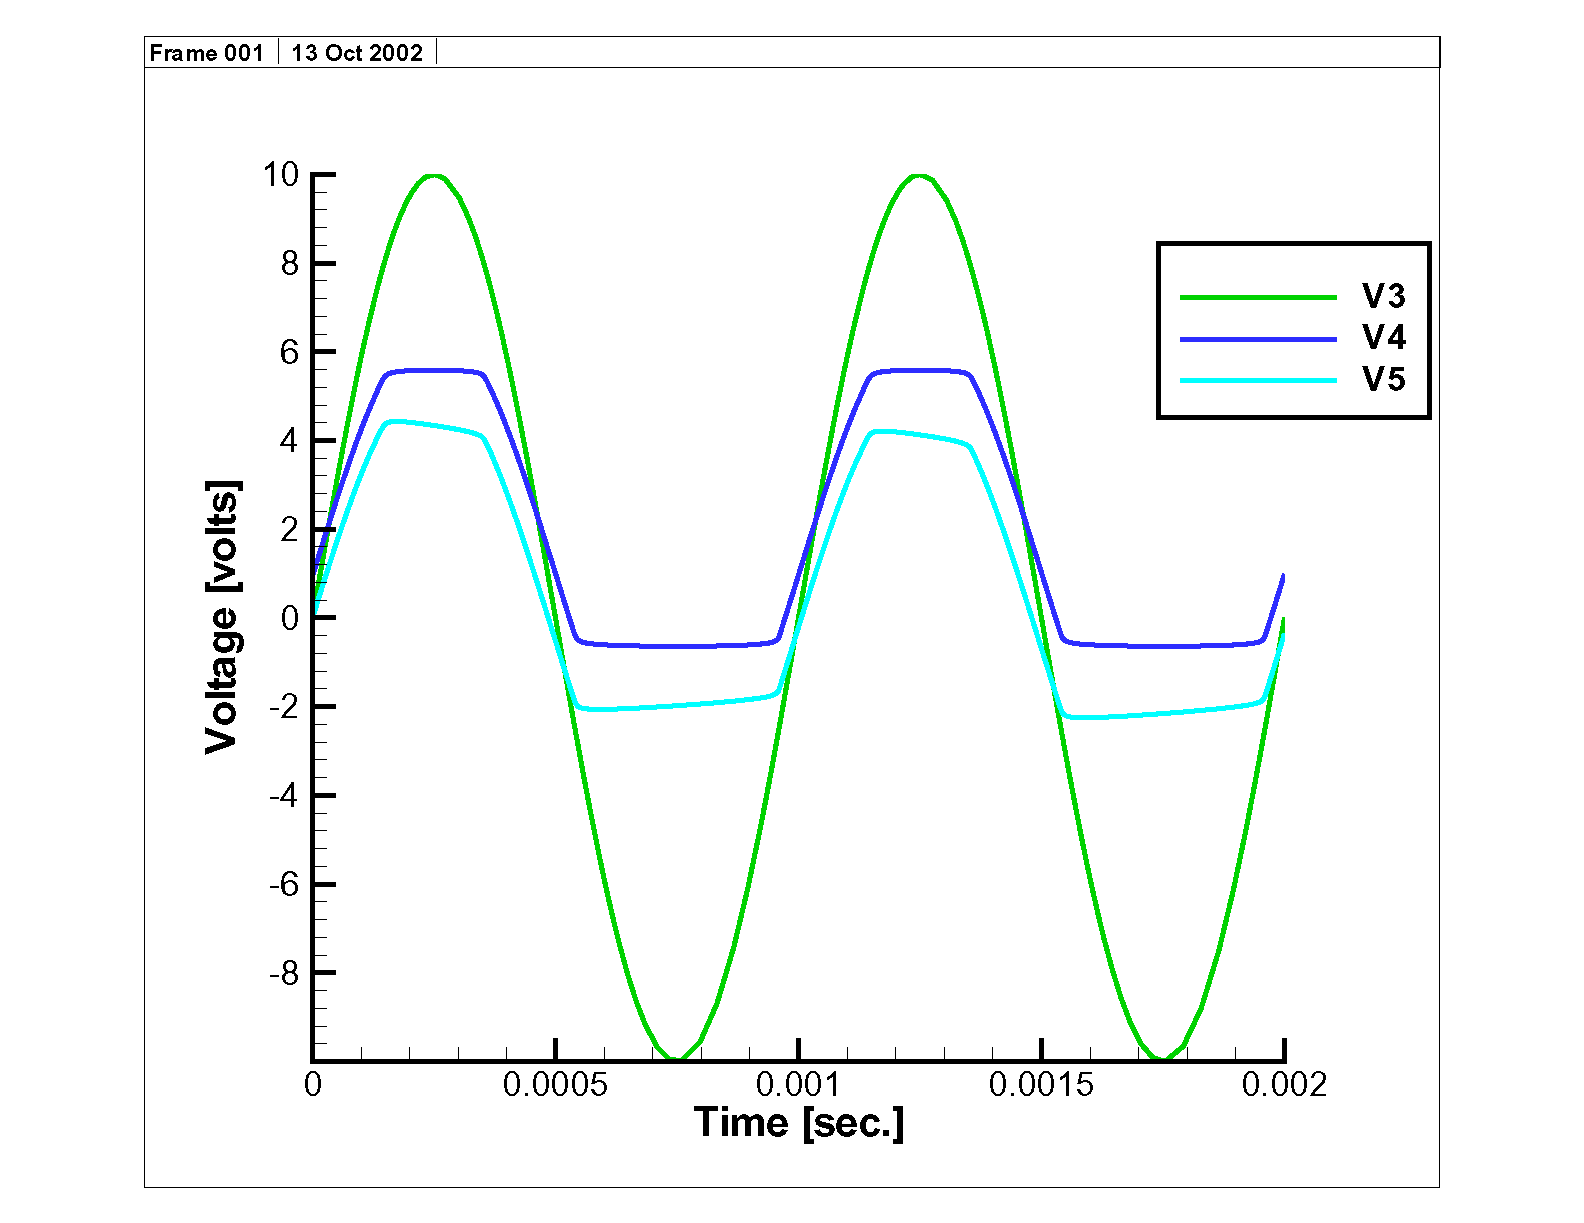
\includegraphics[width=4.5in]{clipper-tp}
      }
    \caption{TecPlot plot of diode clipper circuit transient response from \Xyce{}
      \texttt{.prn} file.\label{Clipper_TP}}
  \end{centering}
\end{figure}

%%% Local Variables:
%%% mode: latex
%%% End:

% END of Xyce_UG_ch12.tex ************
